% =================================================================================================
\chapter{Biološke osnove} % Main chapter title
\label{bioloskeosnove} % For referencing the chapter elsewhere, use \ref{Chapter1} 
% =================================================================================================

U ovoj sekciji biće ukratko predstavljene biološke osnove neophodne za razumevanje rada i motivacije koja stoji iza određenih njegovih elemenata.
Najpre, biće opisano šta su proteini, koje su njihove osnovne funkcije i kakva im je struktura. Potom, biće opisana svaka od struktura ponaosob, uz priložen grafički prikaz istih. Na kraju, posebno će biti opisani neuređeni proteini, njihova uloga i uzroci koji mogu dovesti do njihove pojave. 

% -------------------------------------------------------------------------------------------------
\section{Proteini}
\label{sec:proteini}
% -------------------------------------------------------------------------------------------------

Proteini (grč.~{\em protos} - $"$zauzimam prvo mesto$"$) su biološki makromolekuli neophodni za izgradnju i pravilno funkcionisanje ćelija, i igraju mnogobrojne uloge u različitim procesima koji se odvijaju unutar organizma. Oni su najvažniji sastojak žive materije i utiču na brojnost i raznolikost živih bića. Specifičnost proteina je tolika da svaka biljna i životinjska vrsta ima svoje proteine, a kod viših organizama oni se razlikuju i na individualnom nivou. Broj proteina u živim bićima je ogroman, a kao primer uzmimo $E. coli$ sa $3000$ i čoveka sa $5$ miliona proteina~\cite{spasic}. \\\\
Proteini i peptidi su izgrađeni od $22$\footnote{Neki proteini u svom sastavu mogu da imaju $22$ različite aminokiseline. Pored $20$ “standardnih” aminokiselina,
postoje i $2$ “nestandardne” i to su Selenocistein (eng.~{\em Selenocysteine}, simboli $Sec$, $U$) i Pirolizin (eng.~{\em Pyrrolysine},
simboli $Pyl$, $O$). Ove dve aminokiseline se ređe javljaju~\cite{MarijaJ}.} $L-aminokiseline$ \footnote{$L-aminokiseline$ su one sa levom prostornom konfiguracijom, analogno, postoje i $D-aminokiseline$, sa desnom} koje se javljaju u prirodi i povezani su peptidnim vezama~\cite{biopathways}, koje nastaju između $\alpha$-karboksilne grupe jedne aminokiseline i $\alpha$-amino grupe druge aminokiseline, pri čemu se oslobađa molekul vode~\cite{MarijaJ}. Ovim postupkom nastaje nerazgranati polipeptidni lanac izgrađen od glavnog lanca, koji se pravilno ponavlja, i međusobno različitih ogranaka. $"$Standardna$"$ grupa aminokiselina se može podeliti na esecijalne i
neesecijalne, čiji spisak se može videti u tabeli \ref{table:1}~\cite{MarijaJ}. 
\begin{table}[h!]
\centering
	\begin{tabular}{||c c||} 
	\hline 
	Esencijalne & Neesencijalne \\ [0.5ex] 
	\hline\hline
	Arginin & Alanin \\ 
	\hline
	Histidin & Asparagin \\
	\hline
	Leucin & Asparaginska kiselina\\
	\hline
	Izoleucin & Cistein \\
	\hline
	Lizin & Glutaminska kiselina \\ [1ex] 
	\hline
	Metionin & Glutamin \\ [1ex] 
	\hline
	Fenilalanin & Glicin \\ [1ex] 
	\hline
	Treonin & Prolin \\ [1ex] 
	\hline
	Triptofan & Serin \\ [1ex] 
	\hline
	Valin & Tirozin \\ [1ex] 
	\hline
	\end{tabular}
\caption{Spisak esencijalnih i neesencijalnih aminokiselina}
\label{table:1}
\end{table}
Poznavanje i razumevanje funkcija proteina je esencijalno u istraživanju bilo kog biološkog procesa, sa posebnim naglaskom na oboljenja ljudi, s obzirom da
se mnoga od njih mogu pojaviti zbog funkcionalnih mutacija~\cite{JKd}.\\\\
Svaki molekul proteina nastaje u ćeliji živog organizma. Redosled aminokiselina u proteinskom lancu određen je redosledom nukleotida u dezoksiribonukleinskoj kiselini (DNK). Informacija o broju, vrsti i redosledu aminokiselina zapisana je na delovima DNK koji se nazivaju geni. Svakoj trojci nukleotida u genu na osnovu genetskog koda jedinstveno je pridružena po jedna aminokiselina. U procesu genske ekspresije, posredstvom glasničke
(eng.~{\em messenger}) ribonukleinske kiseline (RNK) i transportne (eng.~{\em transfer}) RNK, enkodirana informacija iz DNK se prevodi u niz aminokiselina u
proteinskom lancu~\cite{JKd}.
Proces sinteze proteina predstavlja \textit{centralnu dogmu molekularne biologije}, čiji se prikaz može videti na slici \ref{fig:dogma}.
\begin{figure}[h]
	\centering
    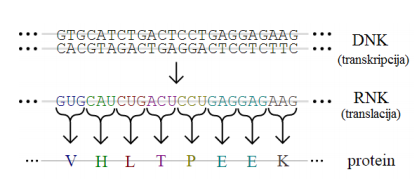
\includegraphics[width=0.5\textwidth]{Figures/BO/dogma.png}
    \caption{Prikaz centralne dogme molekularne biologije~\cite{JKd}}
    \label{fig:dogma}
\end{figure}

\subsection{Funkcije i osobine proteina}
Proteini su biološki najaktivniji molekuli sa velikim brojem esencijalnih uloga koje se dele na:
\begin{itemize}
\item dinamičke, od kojih su najvažnije:
\begin{enumerate} 
\item transportna - prenos molekula (poput kiseonika, gvožđa, lipida) i hormona od mesta sinteze do mesta delovanja,
\item biološka - regulacija metaboličkih procesa u ćeliji, kontrola i regulacija transkripcije gena i translacija,
\item katalizatorska - biološka katalizacija \footnote{Katalizacija predstavlja proces povećavanja brzina reakcija},
\item zaštitna - keratin, koagulacija krvi,
\item održavanje zapremine tečnosti u organizmu,
\end{enumerate}
\item strukturne, od kojih su najvažnije:
\begin{enumerate}
\item obezbeđivanje čvrstine i elastičnosti organa,
\item davanje oblika organizmu,
\item izgradnja strukturnih elemenata ćelije i
\item bitna uloga u kontraktilnim i pokretnim elementima organizma~\cite{spasic}.
\end{enumerate}
\end{itemize} 

Postoji nekoliko osobina koje karakterišu proteine, to su:
\begin{itemize}
\item izgradnja kompleksnih jedinjenja sa različitim supstancama po principu strukturne komplementarnosti i  
\item visoka osetljivost na različite agense koji ih denaturišu \footnote{Denaturacija proteina je proces koji izaziva promene u strukturi proteina menjajući i njihovo fiziološko dejstvo.}. Neki od agenasa su: visoka temperatura, pritisak, mehaničko tretiranje, dejstvo kiselina, baza, organskih rastvarača, materija, itd.~\cite{spasic}.
\end{itemize}
 
\subsection{Struktura proteina}
Struktura proteina zavisi od rasporeda aminokiselina i utiče na njegovu funkciju. Niska aminokiselina sadrži sve potrebne informacije kako bi se formirala trodimenzionalna struktura proteina, za koju se smatra da je najstabilnija~\cite{biopathways}. Ona se formira presavijanjem polipeptidnog lanca na različite načine. Unutrašnjost takve strukture ima visoku gustinu, pa takav lanac ne dopušta promene u sastavu i zahteva prisustvo aminokiselina tačno određene veličine~\cite{spasic}.
Uobičajena raspodela aminokiselina u proteinima je daleko od ravnomerne. Neke aminokiseline se javljaju mnogo češće od ostalih, tako se, na primer, leucin pojavljuje devet puta više od triptofana~\cite{biopathways}. \\\\
Proteinsku strukturu održavaju različite vrste kovalentnih i nekovalentnih interakcija između hemijskih skupina, npr. vodonične, jonske, elektrostatičke, dipolne, itd.. Nabiranjem i uvijanjem lanaca nastaju različiti oblici proteina: vlaknasti, globularni ili eliptični~\cite{medbio}.
Ako mutacija dovede do toga da aminokiselina sa malim bočnim lancem bude zamenjena aminokiselinom sa velikim, pojaviće se problem sa formiranjem trodimenzionalne strukture. Ako bi se, pak, velika aminokiselina zamenila sa malom, pojavio bi se prazan prostor, što bi moglo dovesti do destabilizacije molekula proteina~\cite{spasic}. \\\\
U molekulima proteina postoji hijerarhijska strukturalna organizacija u četiri nivoa:
\begin{enumerate}
\item primarna,
\item sekundarna,
\item tercijarna i
\item kvaternarna~\cite{spasic}.
\end{enumerate}
Na slici \ref{fig:structures} se može videti opšti prikaz mogućih struktura proteina, a na drugoj \ref{fig:structures2} šematski prikaz.
\begin{figure}[h]
	\centering
    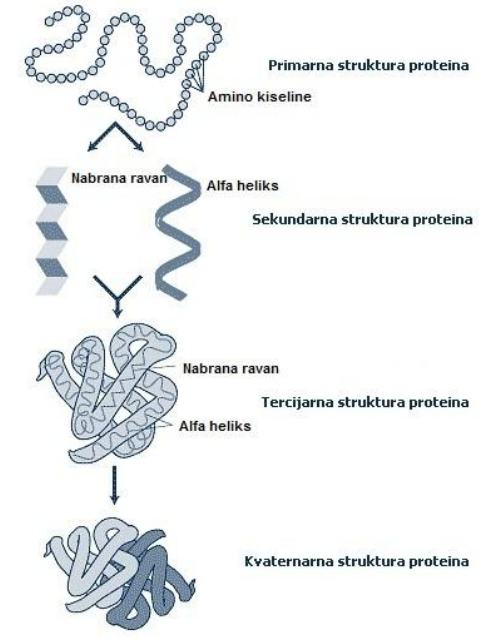
\includegraphics[width=0.5\textwidth]{Figures/BO/protein_structures.png}
    \caption{Prikaz struktura proteina}
    \label{fig:structures}
\end{figure}
\begin{figure}[h]
	\centering
    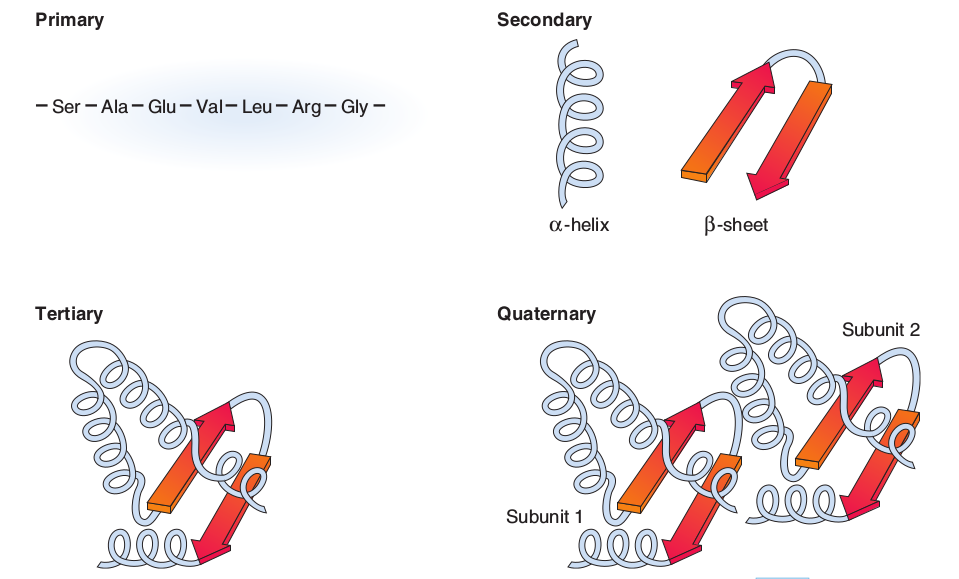
\includegraphics[width=1\textwidth]{Figures/BO/structure_schema.png}
    \caption{Šematski prikaz struktura proteina~\cite{bmbg}}
    \label{fig:structures2}
\end{figure}
\subparagraph{Primarna struktura}
Predstavlja s\^amu sekvencu aminokiselina\footnote{Redosled kojim su aminokiseline poređane u nekom polipeptidu se zove sekvenca aminokiselina~\cite{spasic}.} koje učestvuju u izgradnji proteina. Ona je od ključnog značaja za funkciju proteina zbog interakcija između bočnih lanaca aminokiselina koji određuju trodimenzionalnu strukturu. Proteini koji imaju sličnu sekvencu aminokiselina su $homologi$, a poređenje sekvenci među takvim proteinima može ukazati na genetsku relaciju između različitih vrsta~\cite{spasic}.\\\\
Mnoge genetske bolesti rezultuju u proteinima sa abnormalnim redosledom aminokiselina, što uzrokuje nepravilno presavijanje i gubitak ili nemogućnost normalnog funkcionisanja. Ukoliko su nam poznate strukture normalnih i mutiranih proteina, te informacije možemo iskoristiti za dijagnostikovanje ili proučavanje bolesti~\cite{lippincott}. Primarna struktura će sa mutacijama, u najmanju ruku, izmeniti unos, brisanje ili menjanje aminokiselina. Promene u primarnoj strukturi mogu imati uticaja i na više nivoe proteinskih struktura. Takve promene često dovode do lošeg presavijanja proteina i mogu dovesti do njegovog gubitka funkcije~\cite{flash}.
Prikaz izgleda primarne strukture na primeru insulina kod čoveka se vidi na slici \ref{fig:insulin}.
\begin{figure}[h]
	\centering
    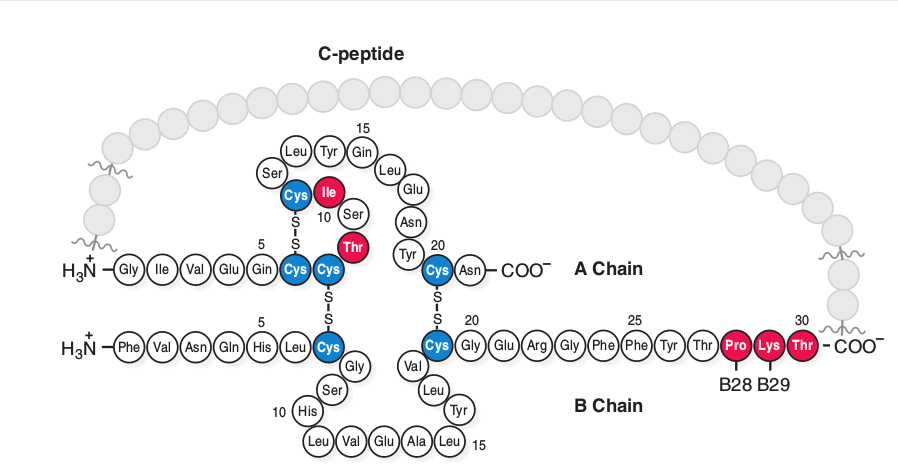
\includegraphics[width=1\textwidth]{Figures/BO/insulin.png}
    \caption{Prikaz primarne strukture~\cite{bmbg}}
    \label{fig:insulin}
\end{figure}
\subparagraph{Sekundarna struktura}
Odnosi se na oblik koji protein zauzima u prostoru i označava pravilno pojavljivanje ponavljanog prostornog rasporeda primarne strukture, u jednoj dimenziji~\cite{medbio}.
Ovu strukturu čini nekoliko različitih oblika, od kojih su najčešći $\alpha$-heliks i $\beta$-presavijena traka (ili $\beta$-struktura), a čest je i tzv. $\beta$-okret~\cite{spasic}.\\\\
\textbf{$\alpha$-heliks} - tip sekundarne strukture kod kog se gusto pakovani polipeptidni lanac spiralno uvrće. Karakteriše se brojem peptidnih jedinica po okretu i rastojanjem između dva okreta. Spada pod energetski najsiromašnije, a time, i najstabilnije strukture proteina. Heliks mogu obrazovati i $L-$ i $D-$ aminokiseline. Postoje dva tipa heliksa: levostrani i desnostrani~\cite{spasic}. Prikaz izgleda $\alpha$-heliksa se vidi na slici \ref{fig:aheliks}.
\begin{figure}[h]
	\centering
    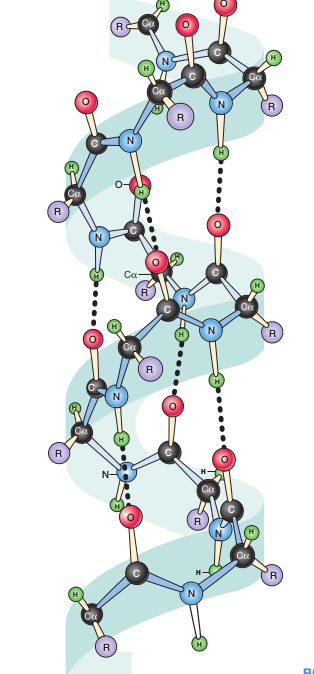
\includegraphics[width=0.25\textwidth]{Figures/BO/ahelix.png}
    \caption{Prikaz $\alpha$-heliksa~\cite{bmbg}}
    \label{fig:aheliks}
\end{figure}
 \\
\textbf{$\beta$-struktura} - Za razliku od $\alpha$-heliksa, sastoji se od dva ili više peptidnih lanaca, ili segmenata polipeptidnih lanaca, a obrazuje se kada se ovakvi tipovi lanca povežu uzdužno. Postoje dva tipa $\beta$-struktura: paralelna i antiparalelna~\cite{spasic}.\\
Prikaz izgleda $\beta$-strukture se vidi na slici \ref{fig:beta}.
\begin{figure}[h]
	\centering
    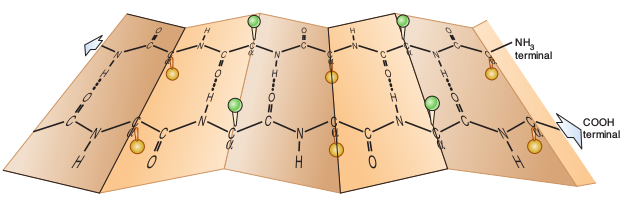
\includegraphics[width=1\textwidth]{Figures/BO/beta.png}
    \caption{Prikaz $\beta$-strukture~\cite{bmbg}}
    \label{fig:beta}
\end{figure}
\textbf{$\beta$-okreti} - obrću pravac polipeptidnog lanca praveći kompaktan globularan oblik~\cite{lippincott}. 
 
Prikaz izgleda sekundarnih struktura se nalazi na slici \ref{fig:ab}.
\begin{figure}[h]
	\centering
    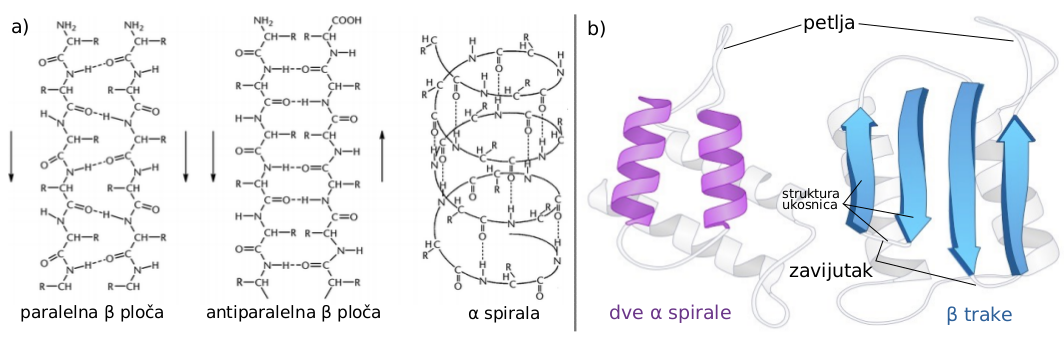
\includegraphics[width=1\textwidth]{Figures/BO/sec_structure.png}
    \caption{Prikaz sekundarnih struktura~\cite{Vinterhalter}}
    \label{fig:ab}
\end{figure}
 

\subparagraph{Tercijarna struktura}
Podrazumeva unutarmolekularno slaganje polipeptidnog lanca u kompaktnu trodimenzionalnu strukturu specifičnog oblika~\cite{medbio}.
Takva trodimenzionalna konformacija nastaje prostornim organizovanjem polipeptidnog lanca koji već ima sekundarnu strukturu. Na taj način se približavaju ostaci aminokiselina koji su udaljeni u primarnoj strukturi. Proteini koji imaju ovakvu strukturu su globularni i kompaktni sa velikom gustinom u središtu~\cite{spasic}.
\subparagraph{Kvaternarna struktura}
Predstavlja agregaciju više peptidnih lanaca u molekulu proteina~\cite{medbio}. Mnogi proteini, posebno oni velike mase, izgrađeni su od nekoliko polipeptidnih lanaca. Svaka takva komponenta naziva se $podjedinica$ ili $protomer$. Oni mogu biti identični\footnote{Tada takve proteine nazivamo $oligomerima$} ili se razlikovati prema strukturi. Ovakav raspored dovodi do brzog i efikasnog transfera substrata od jednog aktivnog centra enzima do drugog~\cite{spasic}.
 
\subsection{Savijanje proteina}
Interakcije između lanaca aminokiselina, koji se nalaze sa strane, određuju kako se dugački polipeptidni lanac presavija u trodimenzionalni oblik funkcionalnog proteina. Presavijanje proteina koje se događa u ćeliji traje od nekoliko sekundi do nekoliko minuta. 
Na slici \ref{fig:folding} se može videti opšti prikaz savijanja proteina.
\begin{figure}[h]
	\centering
    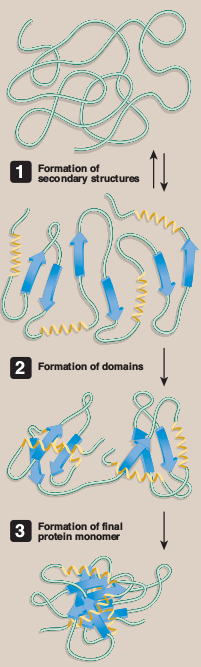
\includegraphics[width=0.25\textwidth]{Figures/BO/protein_folding.png}
    \caption{Prikaz savijanja proteina~\cite{lippincott}}
    \label{fig:folding}
\end{figure}

\subsection{Denaturacija proteina}
Denaturisanje proteina rezultuje u odvijanju i dezorganizaciji proteinske sekundarne i tercijarne strukture. Pod idealnim uslovima, denaturisanje proteina može biti $reverzibilno$. To znači da bi se protein, pri prestanku delovanja agenasa, vratio u normalno stanje. Međutim, većina proteina ostaje trajno neuređena~\cite{lippincott}. O neuređenosti proteina biće više reči u nastavku.\\\\
Jedno od objašnjenja zašto se protein ne vraća u originalno stanje se sastoji u tome da protein počinje sa savijanjem pre nego što se izvrši sinteza celog lanca. Osim toga, specijalizovana grupa pomoćnih proteina (engl. $chaperones$) je neophodna za pravilno savijanje mnogih vrsta proteina. Ovi pomoćni proteini interaguju sa polipeptidima u nekoliko faza tokom procesa savijanja, imaju ulogu u tome da održavaju protein nesavijenim dok sinteza nije gotova, ili imaju ulogu katalizatora~\cite{lippincott}. Loše savijanje proteina može dovesti do različitih bolesti kao što su: amiloidna bolest ili Prionova bolest.
% -------------------------------------------------------------------------------------------------
\section{Neuređenost proteina}
% -------------------------------------------------------------------------------------------------

Neuređenost proteina se utvrđuje eksperimentalno, laboratorijskim analizama, ili uz pomoć prediktora za automatsko utvrđivanje neuređenosti.